\documentclass[11pt, fleqn]{article}

\usepackage{booktabs} % To use /toprule /midrule /bottomrule commands in printing tables
\usepackage{amsmath}
\usepackage{amsfonts}
\usepackage[margin=1in]{geometry} % To set the margin widths
\usepackage{graphicx}
\usepackage{multirow}
\usepackage{tabularx}
\usepackage{tikz}
\usepackage{varioref}
\usepackage{siunitx}

\sisetup{output-exponent-marker=\textsc{e}}

\setlength{\parskip}{12pt} % Sets a blank line in between paragraphs
\setlength\parindent{0pt} % Sets the indent for each paragraph to zero

\begin{document}

\title{Big Data: Homework 2}
\author{Will Clark \& Matthew DeLio \\ Section 01}
\date{\today}
\maketitle

\section{Data Visualization}

We identified three sets of covariates that affect housing prices:
\begin{enumerate}
\item Income/education level: home price tends to rise with income (and with education, which correlates highly with income);
\item Home/neighborhood quality: nice homes and nice neighborhoods demand a price premium; and
\item First-time status: first-time home buyers tend to purchase less expensive homes.
\end{enumerate}

\subsection{Income \& Education}

Unsurprisingly, buyers with higher income and more education are able to afford more expensive homes. We see in Figure~\vref{fig:hhgrad} that the purchase price of a home increases with each additional level of educaiton achieved. In Figure~\vref{fig:income}, we see that home value rises with income, but much of the variation in income is explained by having a college degree. Red dots, signifying purchasers with a college or graduate degree, are concentrated in the northeast corner, signifying high incomes and expensive homes. Blue dots, signifying purchasers without a college degree, have lower incomes and (expectedly) less expensive homes.

\begin{figure}[!htb]
  \centering
  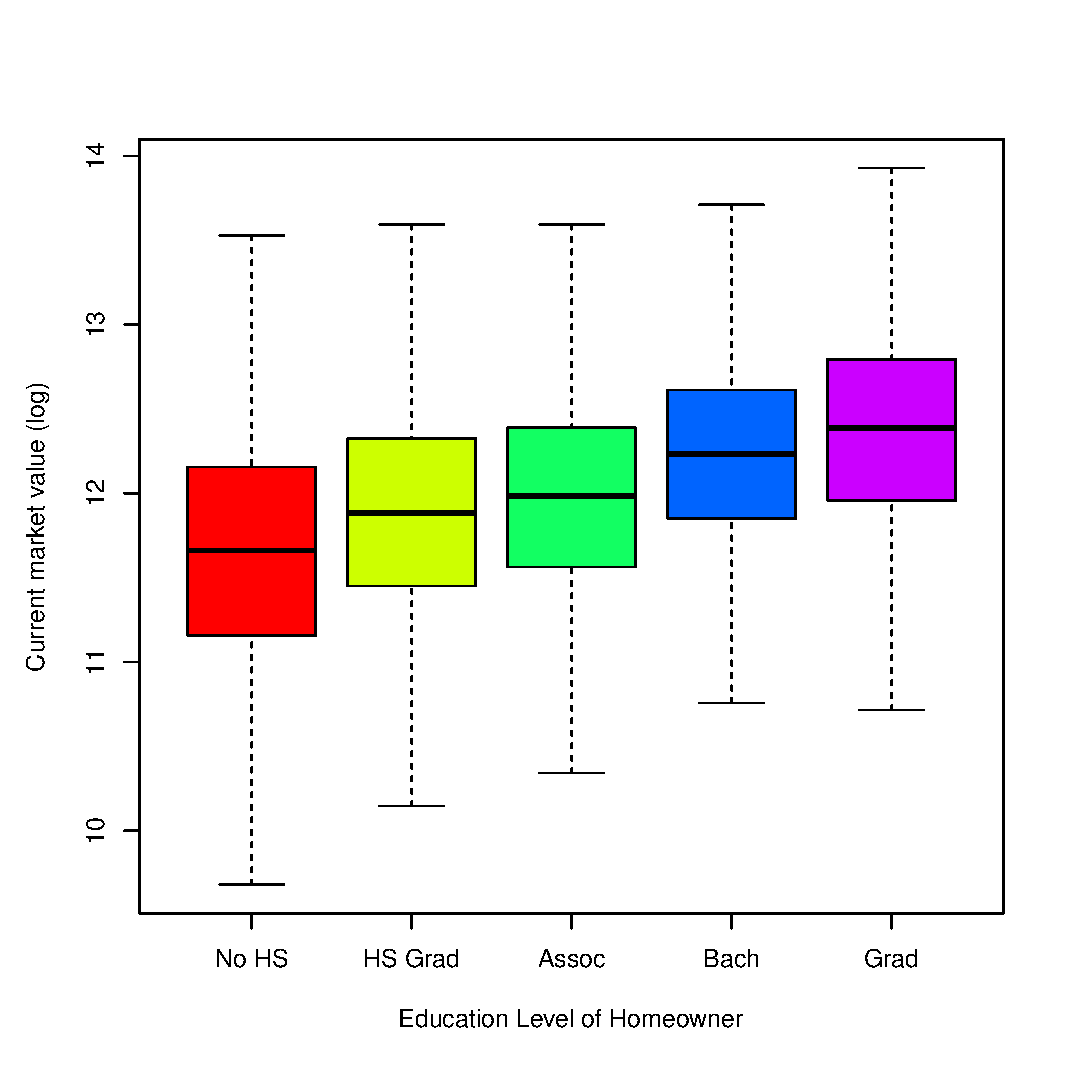
\includegraphics[scale=.5]{hhgrad.eps}
  \caption{Home Value and Education}
  \label{fig:hhgrad}
\end{figure}

\begin{figure}[!htb]
  \centering
  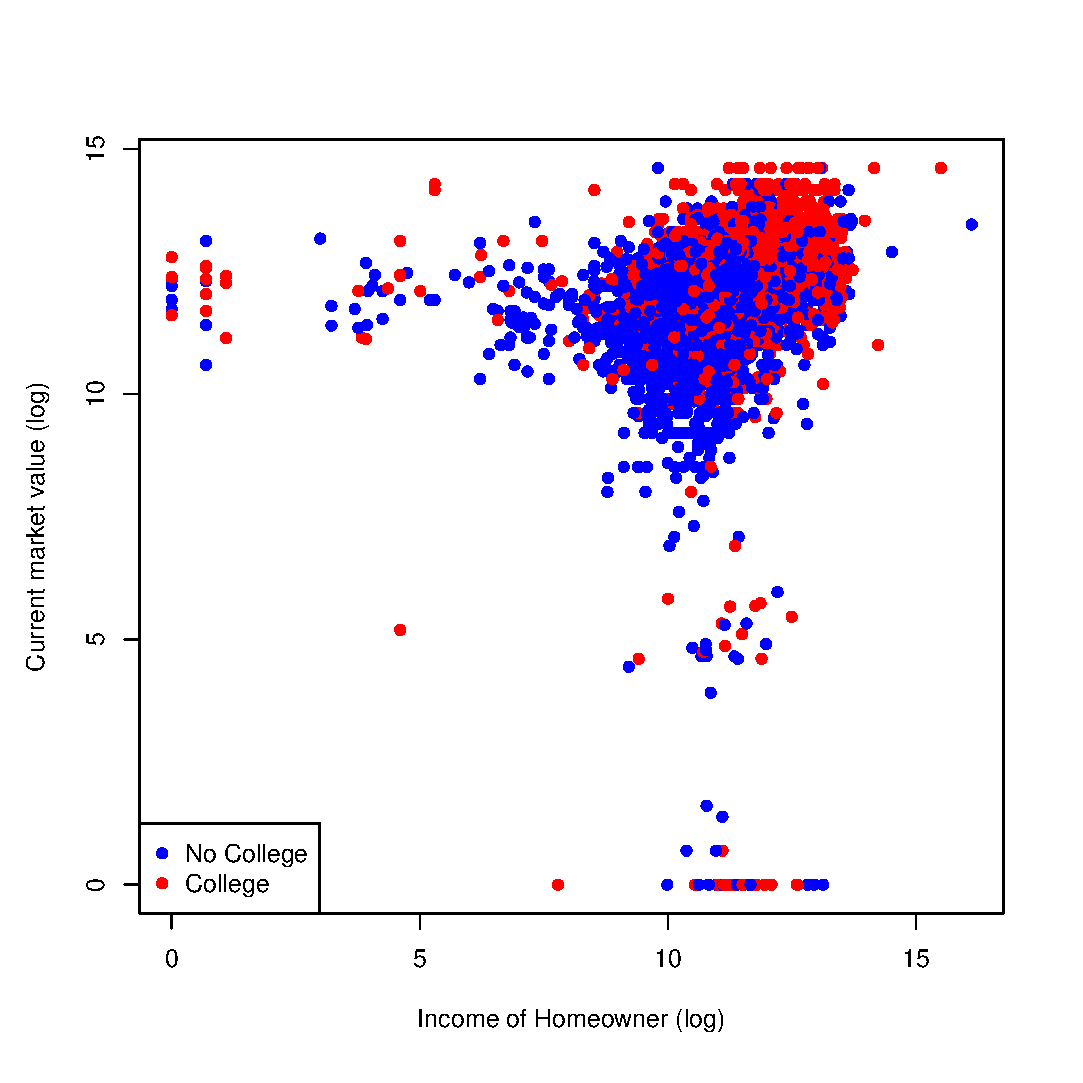
\includegraphics[scale=.5]{income.eps}
  \caption{Home Value and Income}
  \label{fig:income}
\end{figure}

In addition to more expensive homes, more education correlates with neighborhood quality. Figure~\vref{fig:education_qual} shows the share of households by terminal degree level in good and bad neighborhoods. More educated buyers are more likely to have homes in good neighborhoods; we expect that this is really an income story, as education increases income which affords higher neighborhood quality.

\begin{figure}[!htb]
  \centering
  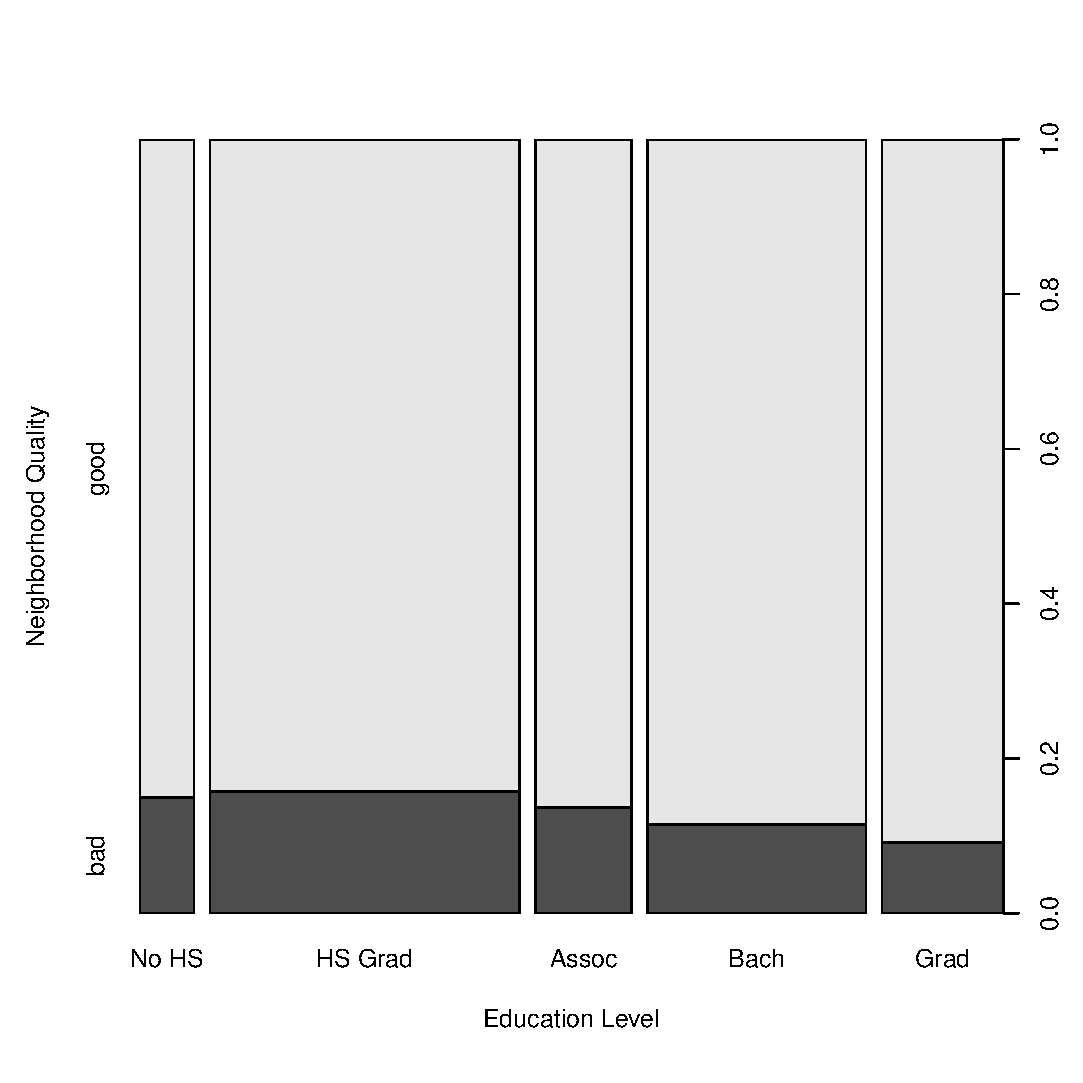
\includegraphics[scale=.5]{neighborhood_quality_vs_education.eps}
  \caption{Neighborhood Quality and Income}
  \label{fig:education_qual}
\end{figure}

\subsection{Neighborhood \& Home}

The value of a home is also driven by the quality of the home and the surrounding neighborhood. We expect that nicer homes in nicer neighborhoods will cost more. We see in Figure~\vref{fig:ejunk} and Figure~\vref{fig:eaban} that two proxies for neighborhood quality\textemdash the presence of junk in the street and proximity to abandoned buldings\textemdash both lower home value. 

\begin{figure}[!htb]
  \centering
  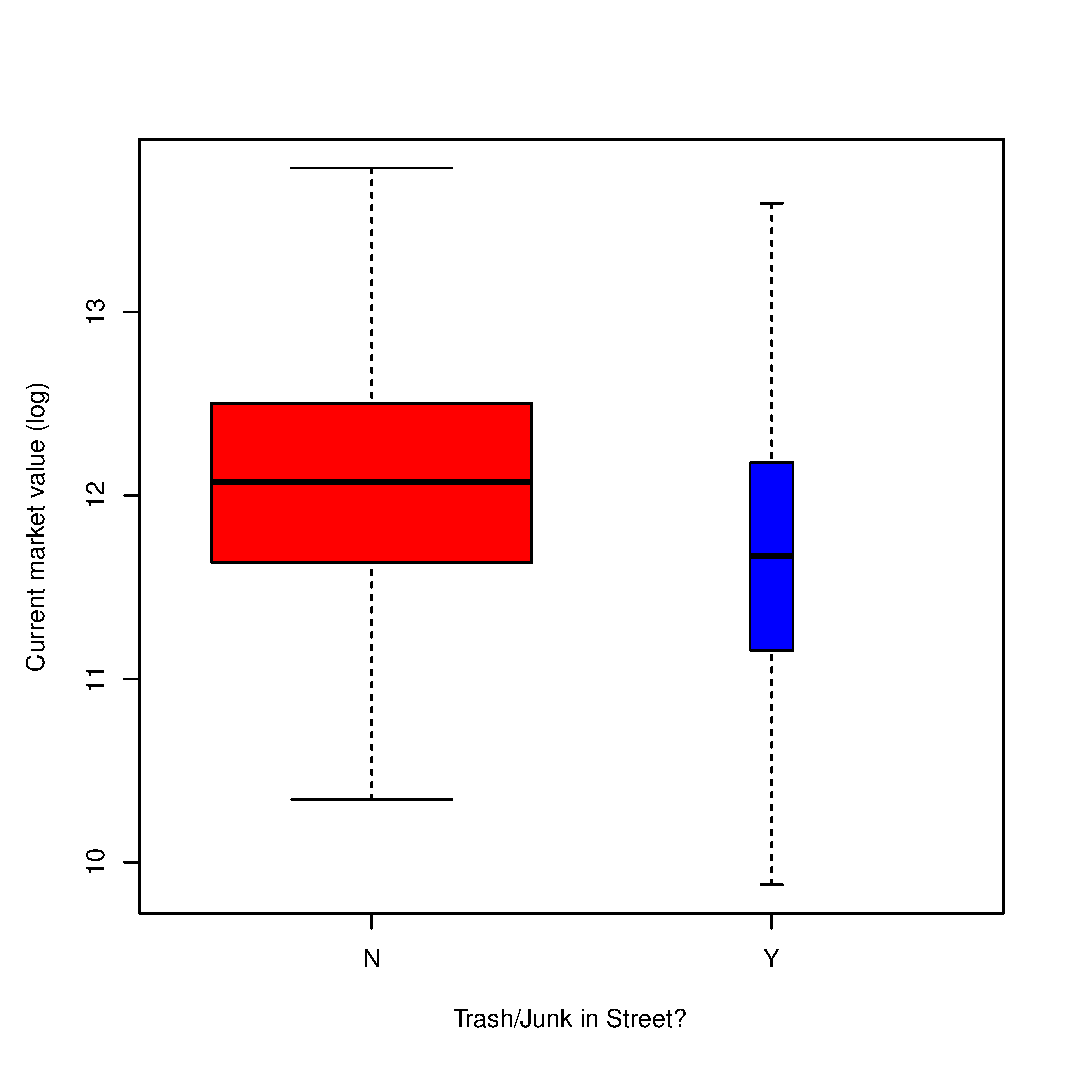
\includegraphics[scale=.5]{ejunk.eps}
  \caption{Near Street Trash}
  \label{fig:ejunk}
\end{figure}

\begin{figure}[!htb]
  \centering
  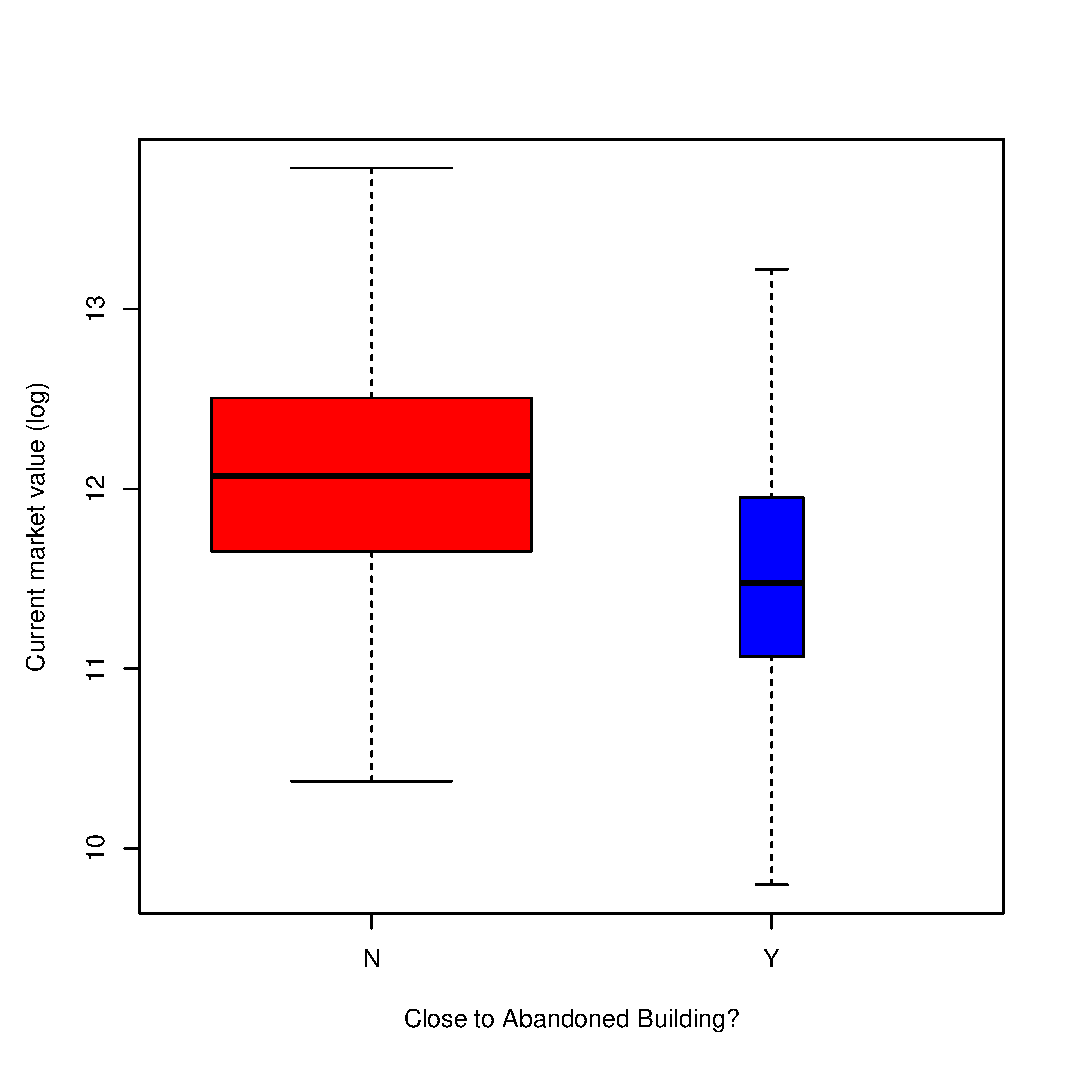
\includegraphics[scale=.5]{eaban.eps}
  \caption{Near Abandoned Buildings}
  \label{fig:eaban}
\end{figure}

As we would expect, homes that are identified as ``good'' quality cost more than those that are not, and good neighborhoods carry a premium over bad neighborhoods (Figure~\ref{fig:howh} and Figure~\ref{fig:hown}, respectively).

\begin{figure}[!htb]
  \centering
  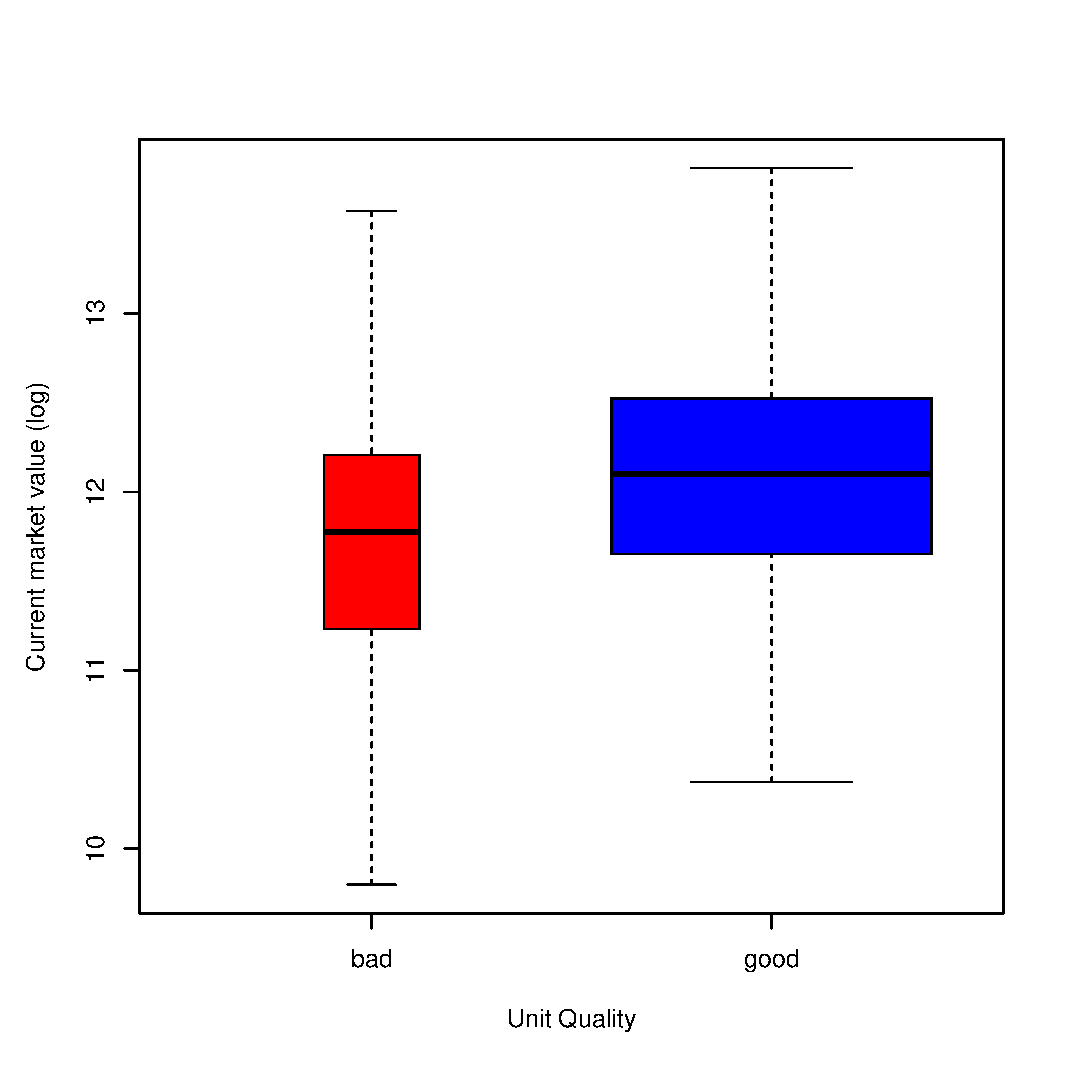
\includegraphics[scale=.5]{howh.eps}
  \caption{Home Quality}
  \label{fig:howh}
\end{figure}

\begin{figure}[!htb]
  \centering
  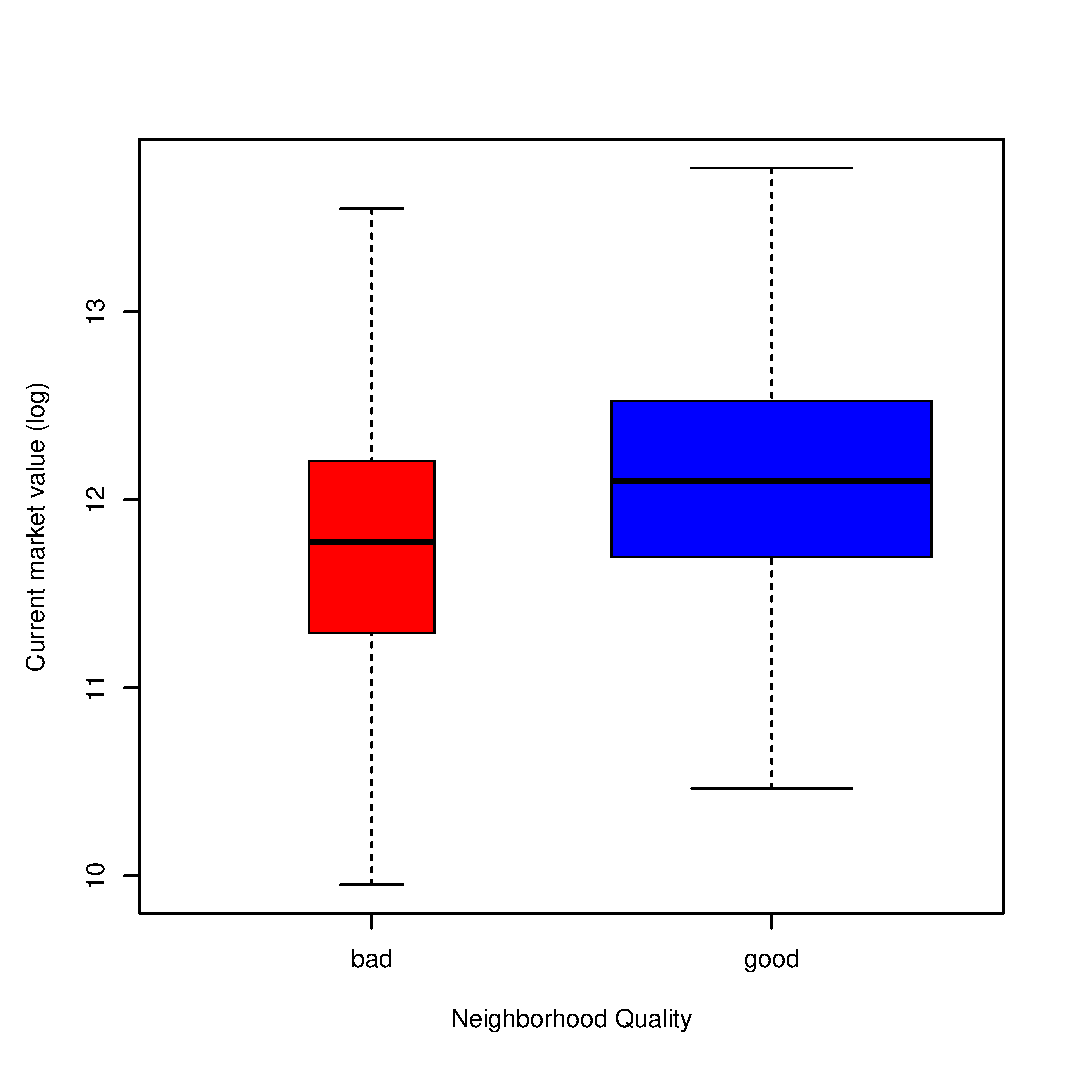
\includegraphics[scale=.5]{hown.eps}
  \caption{Neighborhood Quality}
  \label{fig:hown}
\end{figure}

\begin{figure}[!htb]
  \centering
  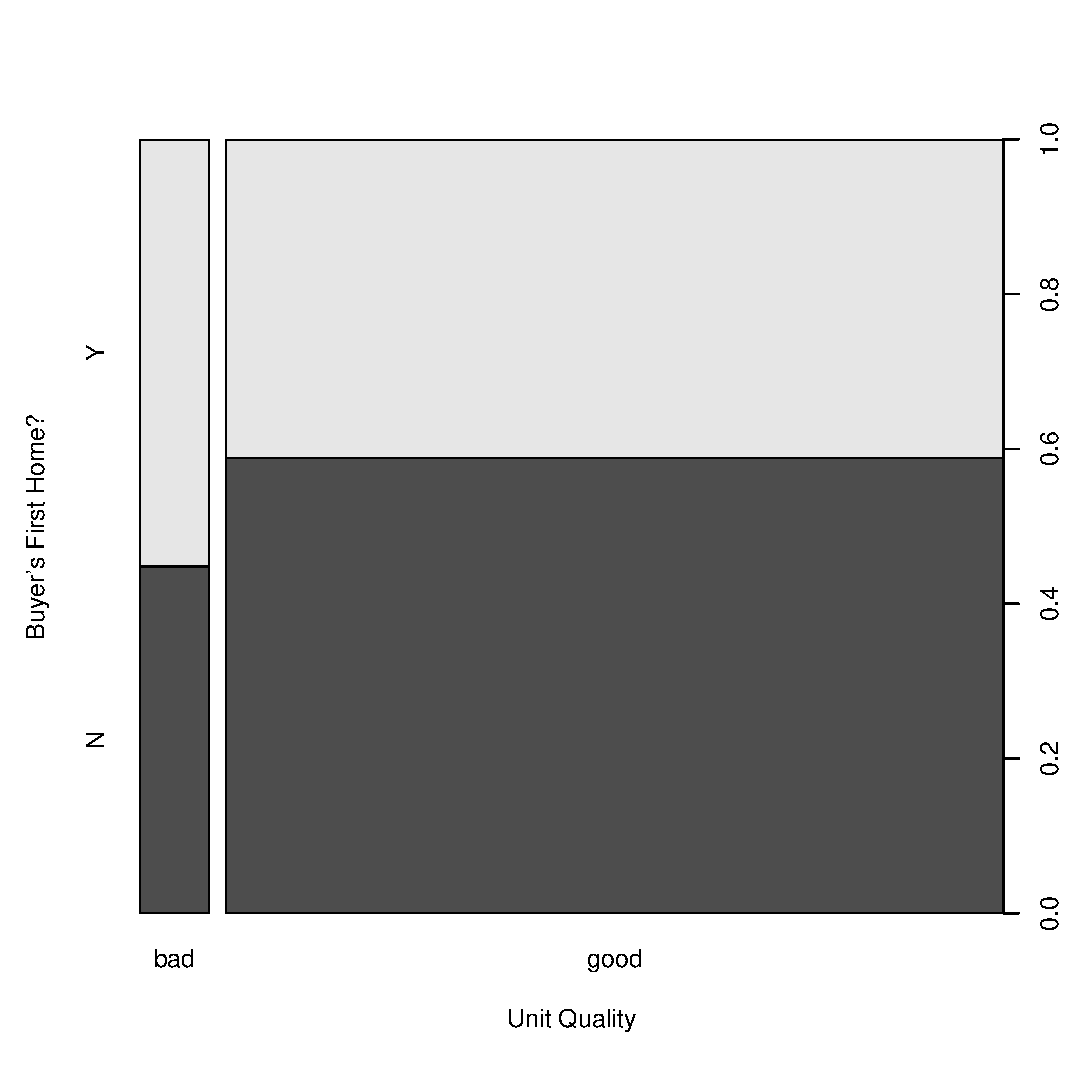
\includegraphics[scale=.5]{first_home_vs_home_quality.eps}
  \caption{}
  \label{fig:first_qual}
\end{figure}

\subsection{First-time Buyers \& Financing Source}

Finally, we examine the difference paid for first-time home buyers versus repeat home buyers. We have two different data sources that tell a similar story. First, buyers who are purchasing their first home tend to pay less than those who are buying a second (or third) home (see Figure~\vref{fig:frstho}). We expect that this is due to age and income differences; first-time home buyers will tend to be younger and have less accumulated wealth than repeat buyers. 

We see that the source of financing for a down payment tells a very similar story. Buyers that use a previous home to pay down their purchase buy more expensive homes (see Figure~\vref{fig:dwnpay}). We expect that this is capturing the same effect as described above: namely, that if a previous home is used as a source of financing, that signals an older buyer with higher income and greater wealth.

\begin{figure}[!htb]
  \centering
  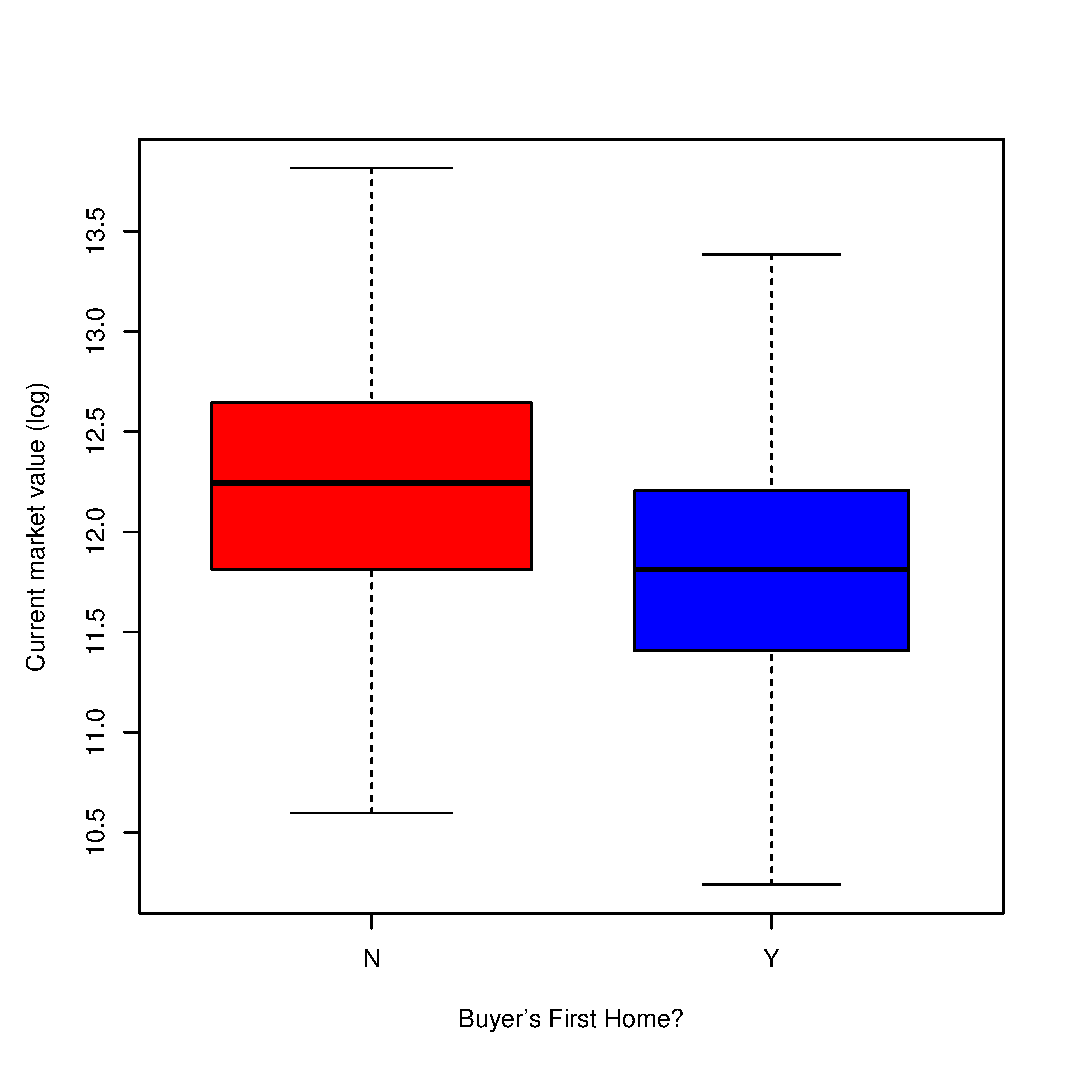
\includegraphics[scale=.5]{frstho.eps}
  \caption{First Time Buyers}
  \label{fig:frstho}
\end{figure}

\begin{figure}[!htb]
  \centering
  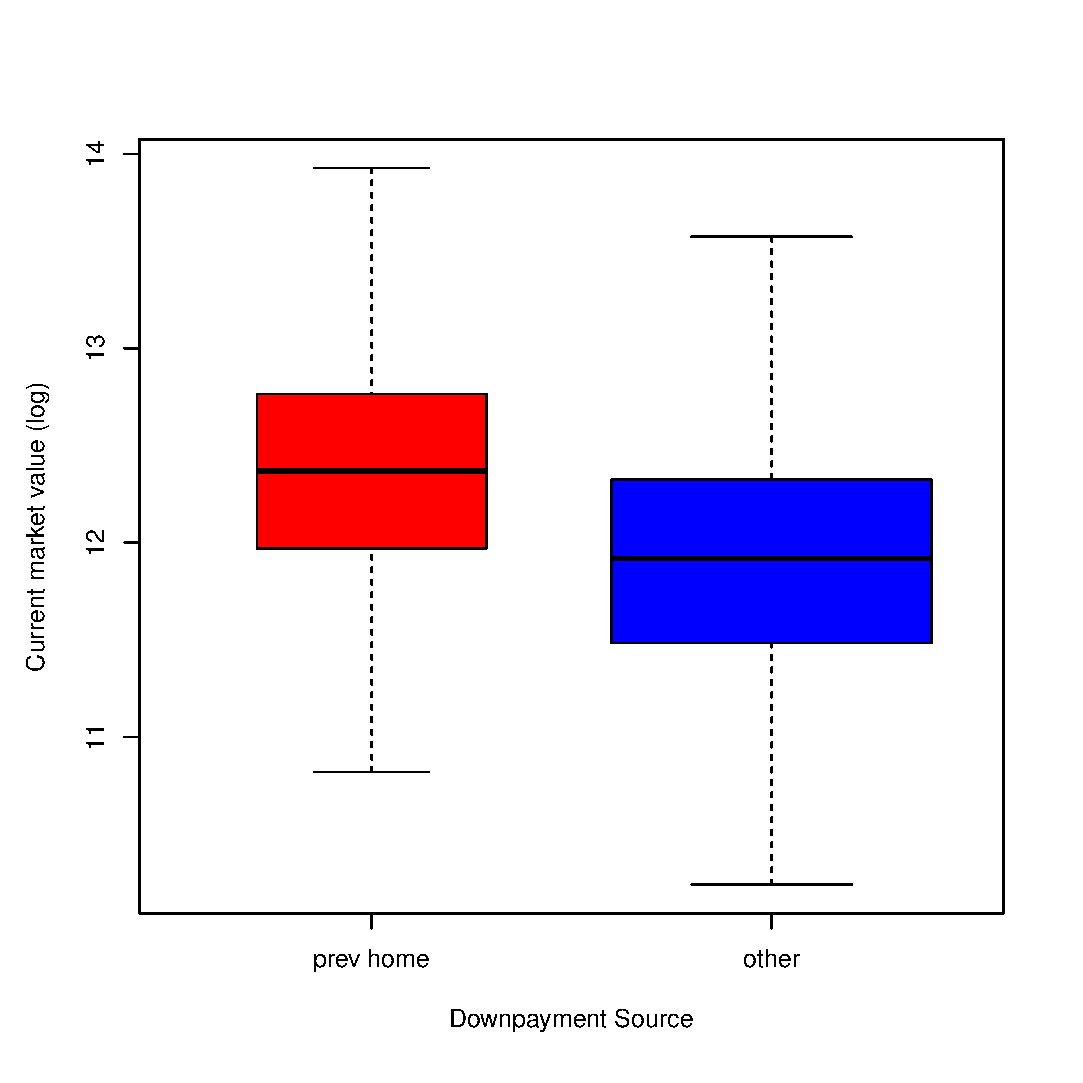
\includegraphics[scale=.5]{dwnpay.eps}
  \caption{Mortgage Financing}
  \label{fig:dwnpay}
\end{figure}

\section{Linear Model}
% latex table generated in R 3.1.2 by xtable 1.7-4 package
% Thu Apr 16 19:27:00 2015
\begin{table}[ht]
\centering
\begin{tabular}{rrrrr}
  \hline
 & Estimate & Std. Error & t value & Pr($>$$|$t$|$) \\ 
  \hline
(Intercept) & 11.5901 & 0.0606 & 191.21 & 0.0000 \\ 
  EAPTBLY & -0.0446 & 0.0221 & -2.02 & 0.0436 \\ 
  ECOM2Y & -0.0985 & 0.0470 & -2.10 & 0.0361 \\ 
  EJUNKY & -0.1258 & 0.0509 & -2.47 & 0.0134 \\ 
  ESFDY & 0.2884 & 0.0292 & 9.86 & 0.0000 \\ 
  EABANY & -0.1633 & 0.0359 & -4.55 & 0.0000 \\ 
  HOWHgood & 0.1292 & 0.0263 & 4.92 & 0.0000 \\ 
  HOWNgood & 0.1197 & 0.0219 & 5.47 & 0.0000 \\ 
  STRNAY & -0.0391 & 0.0158 & -2.47 & 0.0136 \\ 
  ZINC2 & 0.0000 & 0.0000 & 11.24 & 0.0000 \\ 
  HHGRADBach & 0.1333 & 0.0229 & 5.82 & 0.0000 \\ 
  HHGRADGrad & 0.1979 & 0.0257 & 7.69 & 0.0000 \\ 
  `HHGRADHS Grad` & -0.0615 & 0.0217 & -2.84 & 0.0046 \\ 
  `HHGRADNo HS` & -0.1971 & 0.0318 & -6.20 & 0.0000 \\ 
  NUNITS & -0.0010 & 0.0005 & -1.87 & 0.0610 \\ 
  INTW & -0.0469 & 0.0044 & -10.66 & 0.0000 \\ 
  METROurban & 0.0837 & 0.0179 & 4.67 & 0.0000 \\ 
  STATECO & -0.2876 & 0.0290 & -9.91 & 0.0000 \\ 
  STATECT & -0.3444 & 0.0312 & -11.04 & 0.0000 \\ 
  STATEGA & -0.6555 & 0.0309 & -21.20 & 0.0000 \\ 
  STATEIL & -0.8624 & 0.0576 & -14.96 & 0.0000 \\ 
  STATEIN & -0.7779 & 0.0307 & -25.37 & 0.0000 \\ 
  STATELA & -0.7218 & 0.0368 & -19.63 & 0.0000 \\ 
  STATEMO & -0.6647 & 0.0334 & -19.89 & 0.0000 \\ 
  STATEOH & -0.6762 & 0.0326 & -20.73 & 0.0000 \\ 
  STATEOK & -0.9978 & 0.0328 & -30.43 & 0.0000 \\ 
  STATEPA & -0.8681 & 0.0338 & -25.67 & 0.0000 \\ 
  STATETX & -1.0497 & 0.0343 & -30.64 & 0.0000 \\ 
  STATEWA & -0.1203 & 0.0309 & -3.89 & 0.0001 \\ 
  BATHS & 0.2134 & 0.0116 & 18.46 & 0.0000 \\ 
  BEDRMS & 0.0877 & 0.0094 & 9.35 & 0.0000 \\ 
  MATBUYY & -0.0277 & 0.0136 & -2.03 & 0.0421 \\ 
  `DWNPAYprev home` & 0.1215 & 0.0178 & 6.81 & 0.0000 \\ 
  FRSTHOY & -0.0829 & 0.0172 & -4.82 & 0.0000 \\ 
   \hline
\end{tabular}
\caption{Value of Purchased Homes (in logs)} 
\label{tab:reg1_fdr}
\end{table}


hi

\section{Logit Model}

\subsection{Interpret Effects}
% latex table generated in R 3.1.2 by xtable 1.7-4 package
% Fri Apr 17 00:56:45 2015
\begin{table}[ht]
\centering
\begin{tabular}{rrrrr}
  \hline
 & Estimate & Std. Error & t value & Pr($>$$|$t$|$) \\ 
  \hline
(Intercept) & 0.1925 & 0.0261 & 7.37 & 0.0000 \\ 
  ECOM1Y & -0.0285 & 0.0096 & -2.96 & 0.0031 \\ 
  ECOM2Y & -0.0439 & 0.0248 & -1.77 & 0.0763 \\ 
  ESFDY & -0.0566 & 0.0151 & -3.74 & 0.0002 \\ 
  HOWNgood & 0.0166 & 0.0105 & 1.59 & 0.1122 \\ 
  STRNAY & -0.0164 & 0.0083 & -1.97 & 0.0489 \\ 
  PER & -0.0208 & 0.0025 & -8.34 & 0.0000 \\ 
  HHGRADBach & 0.0354 & 0.0082 & 4.31 & 0.0000 \\ 
  HHGRADGrad & 0.0563 & 0.0103 & 5.45 & 0.0000 \\ 
  INTW & -0.0094 & 0.0023 & -4.11 & 0.0000 \\ 
  STATECT & 0.1423 & 0.0128 & 11.08 & 0.0000 \\ 
  STATEGA & -0.0476 & 0.0130 & -3.66 & 0.0003 \\ 
  STATEIL & 0.1045 & 0.0286 & 3.66 & 0.0003 \\ 
  STATEIN & 0.0332 & 0.0127 & 2.61 & 0.0091 \\ 
  STATELA & 0.0953 & 0.0166 & 5.73 & 0.0000 \\ 
  STATEMO & 0.0926 & 0.0146 & 6.36 & 0.0000 \\ 
  STATEOH & 0.1342 & 0.0139 & 9.63 & 0.0000 \\ 
  STATEPA & 0.1028 & 0.0148 & 6.96 & 0.0000 \\ 
  STATETX & 0.0406 & 0.0148 & 2.75 & 0.0059 \\ 
  BATHS & 0.0433 & 0.0058 & 7.49 & 0.0000 \\ 
  MATBUYY & 0.0493 & 0.0071 & 6.94 & 0.0000 \\ 
  `DWNPAYprev home` & 0.1605 & 0.0094 & 17.15 & 0.0000 \\ 
  VALUE & 0.0000 & 0.0000 & 12.89 & 0.0000 \\ 
  FRSTHOY & -0.0579 & 0.0090 & -6.43 & 0.0000 \\ 
   \hline
\end{tabular}
\caption{Probability of Down Payment $>$ 20\% (No Interaction Terms)} 
\label{tab:reg3_fdr}
\end{table}


\subsection{Interpret Interaction}
% latex table generated in R 3.1.2 by xtable 1.7-4 package
% Thu Apr 16 19:10:20 2015
\begin{table}[ht]
\centering
\begin{tabular}{rrrrr}
  \hline
 & Estimate & Std. Error & t value & Pr($>$$|$t$|$) \\ 
  \hline
(Intercept) & 0.1766 & 0.0255 & 6.92 & 0.0000 \\ 
  ECOM1Y & -0.0284 & 0.0096 & -2.94 & 0.0032 \\ 
  ECOM2Y & -0.0449 & 0.0248 & -1.81 & 0.0700 \\ 
  ESFDY & -0.0573 & 0.0151 & -3.79 & 0.0002 \\ 
  HOWNgood & 0.0174 & 0.0105 & 1.67 & 0.0957 \\ 
  STRNAY & -0.0166 & 0.0083 & -1.99 & 0.0462 \\ 
  PER & -0.0208 & 0.0025 & -8.35 & 0.0000 \\ 
  HHGRADBach & 0.0358 & 0.0082 & 4.36 & 0.0000 \\ 
  HHGRADGrad & 0.0566 & 0.0103 & 5.48 & 0.0000 \\ 
  INTW & -0.0097 & 0.0023 & -4.22 & 0.0000 \\ 
  STATECT & 0.1411 & 0.0128 & 11.00 & 0.0000 \\ 
  STATEGA & -0.0473 & 0.0130 & -3.64 & 0.0003 \\ 
  STATEIL & 0.1024 & 0.0286 & 3.59 & 0.0003 \\ 
  STATEIN & 0.0324 & 0.0127 & 2.55 & 0.0109 \\ 
  STATELA & 0.0955 & 0.0166 & 5.74 & 0.0000 \\ 
  STATEMO & 0.0910 & 0.0145 & 6.25 & 0.0000 \\ 
  STATEOH & 0.1324 & 0.0139 & 9.50 & 0.0000 \\ 
  STATEPA & 0.0999 & 0.0148 & 6.77 & 0.0000 \\ 
  STATETX & 0.0397 & 0.0147 & 2.69 & 0.0071 \\ 
  BATHS & 0.0556 & 0.0058 & 9.52 & 0.0000 \\ 
  MATBUYY & 0.0493 & 0.0071 & 6.95 & 0.0000 \\ 
  `DWNPAYprev home` & 0.1553 & 0.0092 & 16.84 & 0.0000 \\ 
  VALUE & 0.0000 & 0.0000 & 12.35 & 0.0000 \\ 
  `BATHS:FRSTHOY` & -0.0367 & 0.0047 & -7.75 & 0.0000 \\ 
   \hline
\end{tabular}
\caption{Probability of Down Payment $>$ 20\% (With Interaction Term)} 
\label{tab:reg4_fdr}
\end{table}


\section{Out-of-Sample Prediction}
\subsection{Predicting Downpayments on Homes $<$100k}
\begin{figure}[!htb]
  \centering
  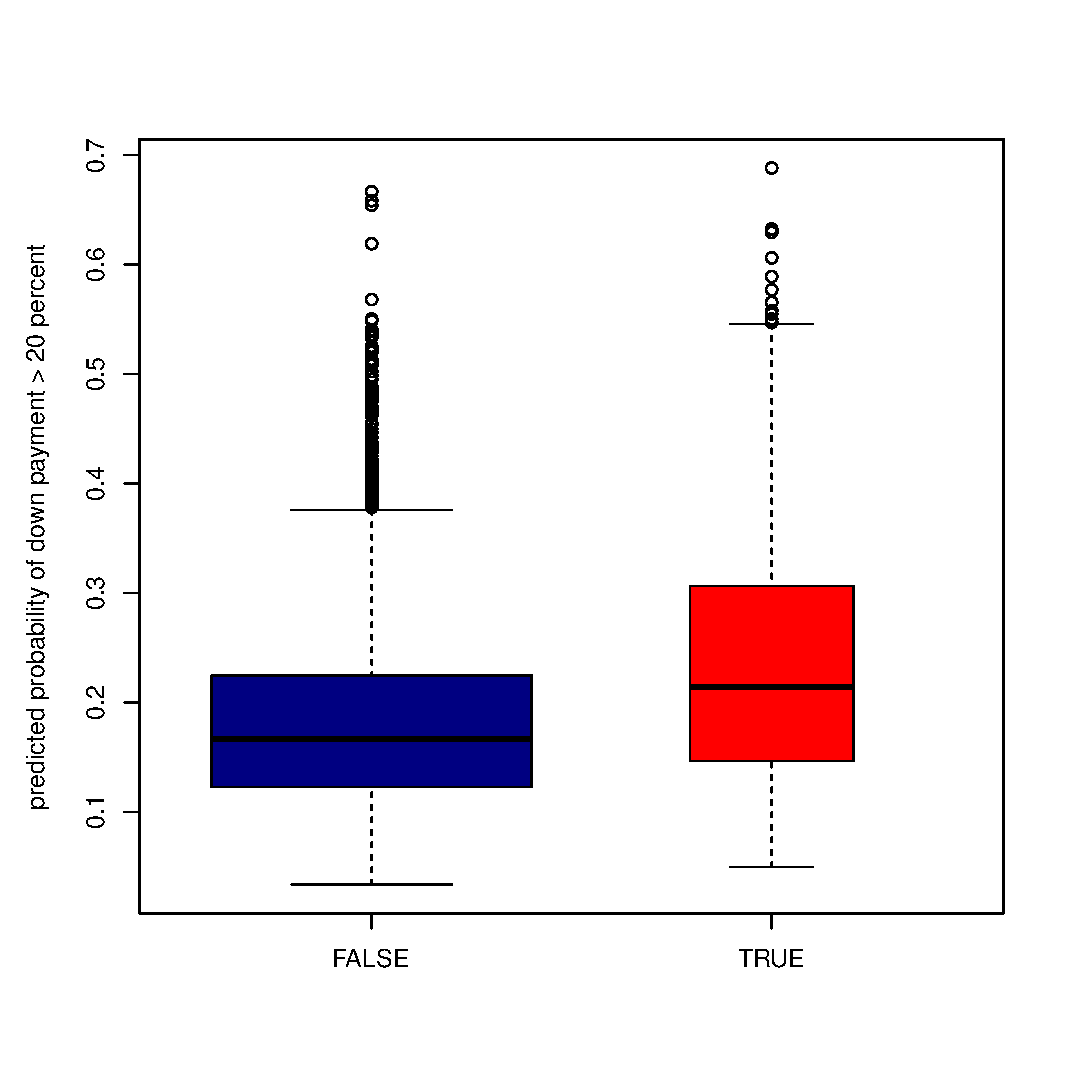
\includegraphics[scale=.5]{oos_lt100k.eps}
  \caption{}
  \label{fig:oos_lt100k}
\end{figure}

\begin{figure}[!htb]
  \centering
  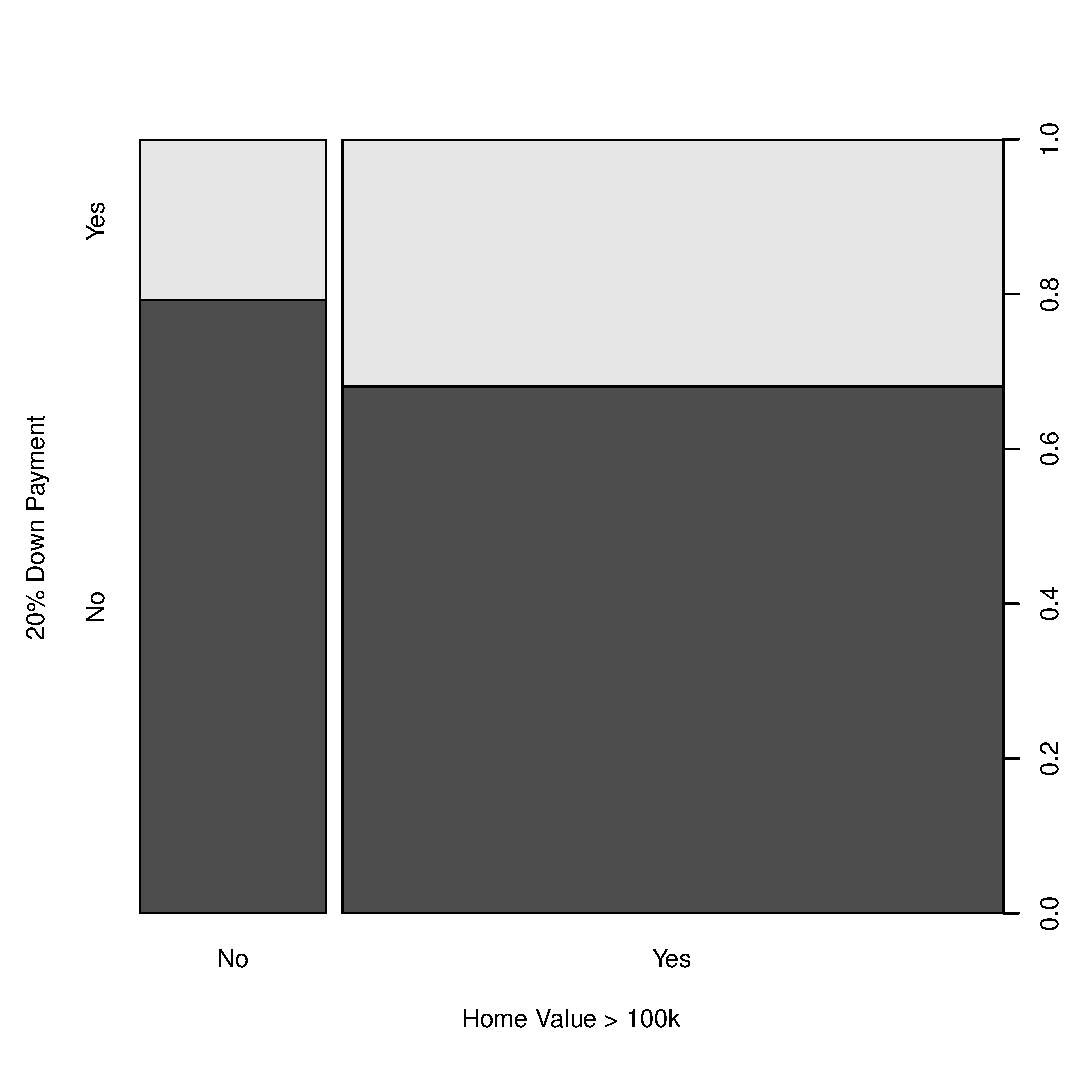
\includegraphics[scale=.5]{home_value_vs_20_down.eps}
  \caption{}
  \label{fig:value_20dwn}
\end{figure}

\subsection{Sample Predictions on Homes $>$100k}

\begin{figure}[!htb]
  \centering
  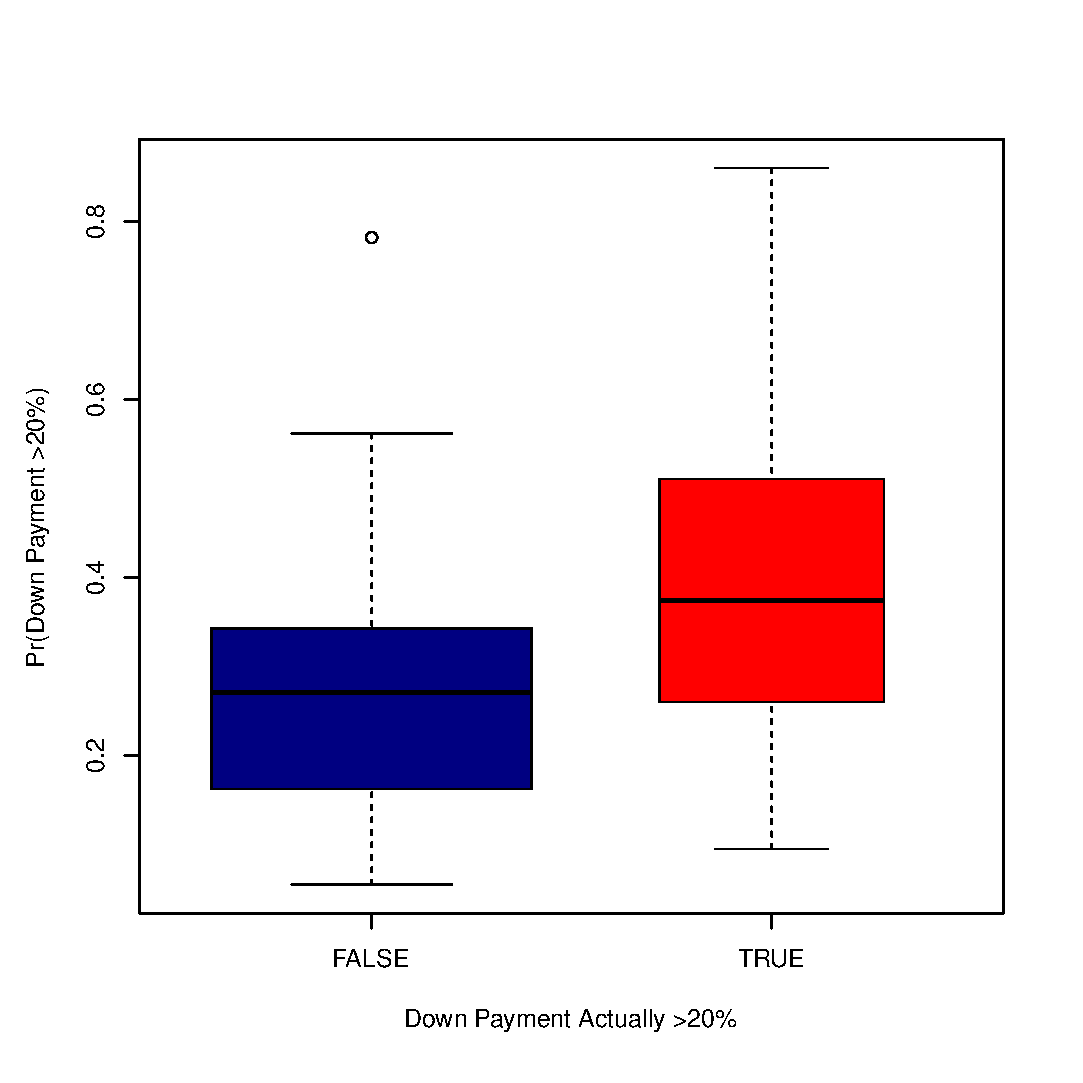
\includegraphics[scale=.5]{oos_subsample_100k.eps}
  \caption{}
  \label{fig:oos_sample_gt100k}
\end{figure}

\end{document}
